
\begin{frame}{\citetitle{ProyectoRefrigeradoresFrios_2022}$^*$ (1)}
\begin{columns}
\begin{column}{0.65\textwidth}
	\begin{itemize}  %del cuerpo académico Acuicultura Sustentable (UTMTB-CA-1)
        \item La Secretaría de Salud del de Tamaulipas almacena en refrigeradores y cámaras frías biológico (vacunas)
        \item Personal de las unidades de salud realiza registros y emite alarmas en situaciones anómalas
		\item Se propone un sistema capaz de vigilar remotamente (24/7) las variables de temperatura, humedad y conexión a la red eléctrica
	\end{itemize}
\end{column}
\begin{column}{0.35\textwidth}  
\begin{center}
     \begin{tabular}{cc}
         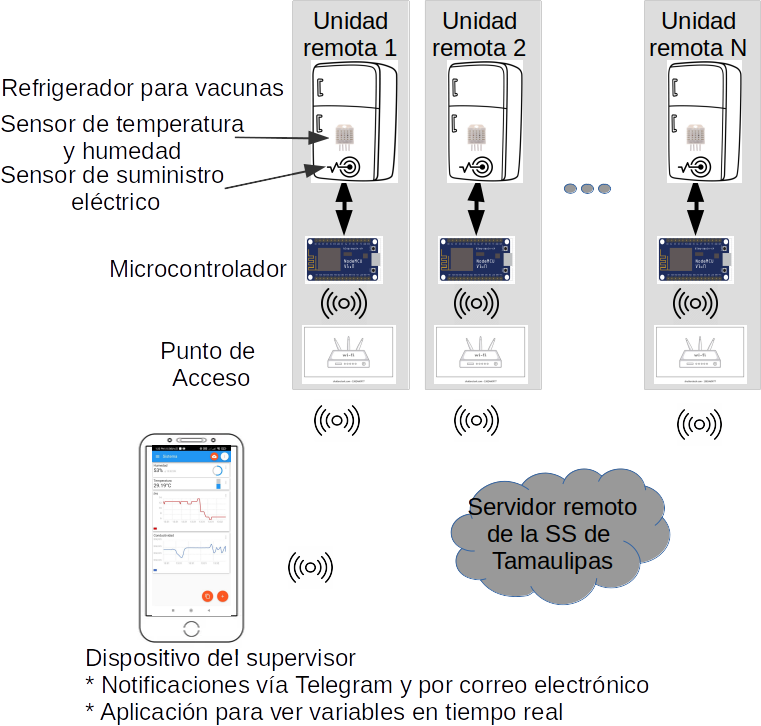
\includegraphics[width=0.98\textwidth]{2022_RefrigeradoresFrios/figs/SistemaRefrigeradoresFrios}\\         
      \end{tabular}
\end{center}
\end{column} 
\end{columns} 
\footfullcite*{ProyectoRefrigeradoresFrios_2022}
\end{frame}


\begin{frame}{\citetitle{ProyectoRefrigeradoresFrios_2022} (2)}
\begin{columns}
\begin{column}{0.8\textwidth}
Resultados:
\begin{itemize}
    \item Se construyeron 325 dispositivos sensores, un sistema de información (para monitorear alarmas y valores de los sensores en rangos específicos de tiempo) y una aplicación movil
    \item Se han instalado dispositivos de monitoreo en 109 de 321 refrigeradores de la SST en 32 municipios de Tamaulipas
    \item Al cierre de esta presentación, se generaron más de 200 alarmas que han obligado a los responsables a verificar el estado de los refrigeradores
	\end{itemize}
\end{column}
\begin{column}{0.2\textwidth}  
\begin{center}
     \begin{tabular}{c}
         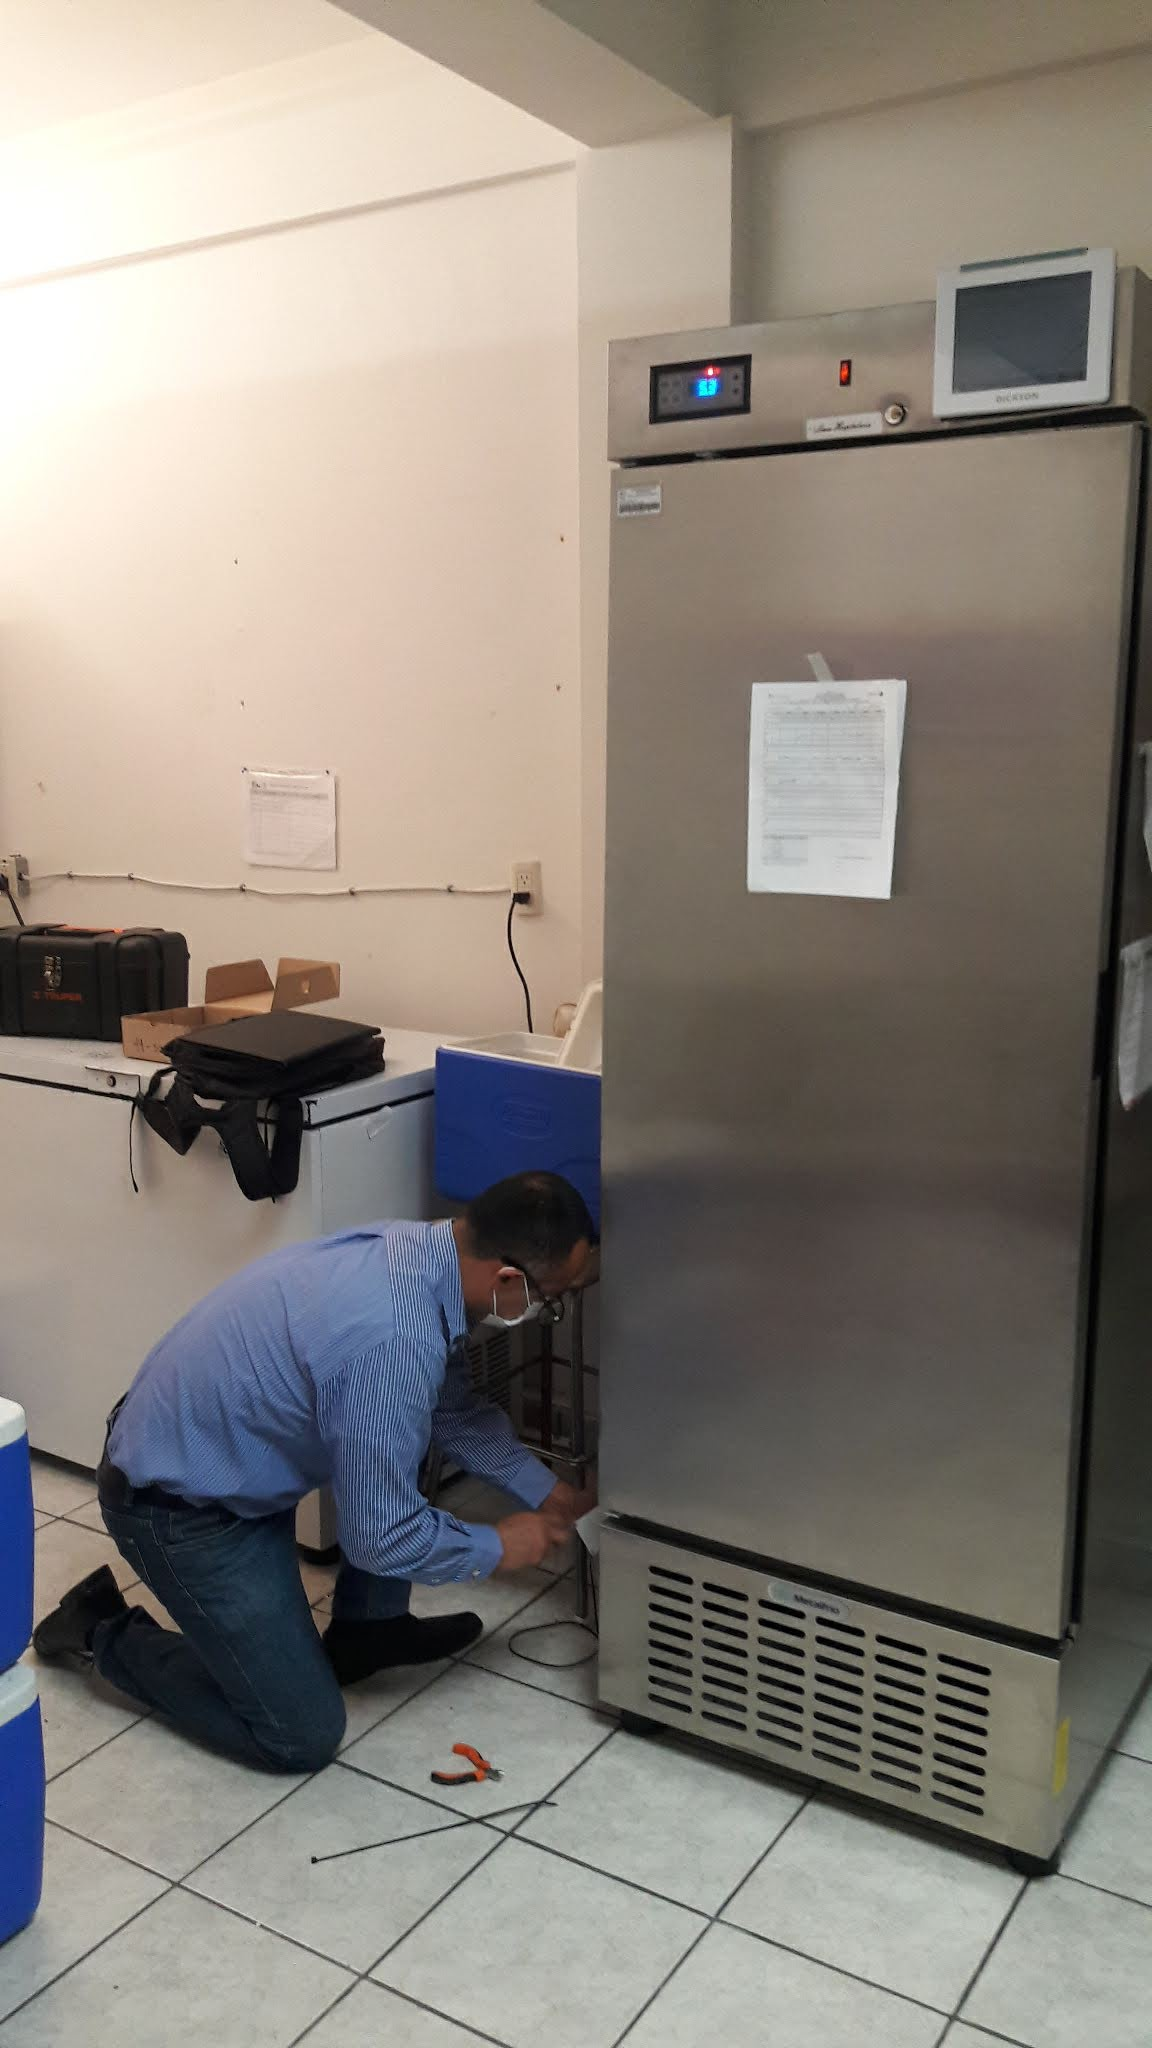
\includegraphics[width=0.98\textwidth]{2022_RefrigeradoresFrios/figs/RefrisSST}\\
          \end{tabular}
\end{center}
\end{column} 
\end{columns} 
\end{frame}




